\documentclass{article}
\usepackage[final]{nips_2017}
\usepackage[utf8]{inputenc} % allow utf-8 input
\usepackage[T1]{fontenc}    % use 8-bit T1 fonts
\usepackage{hyperref}       % hyperlinks
\usepackage{url}            % simple URL typesetting
\usepackage{booktabs}       % professional-quality tables
\usepackage{amsfonts}       % blackboard math symbols
\usepackage{nicefrac}       % compact symbols for 1/2, etc.
\usepackage{microtype}      % microtypography
\usepackage{graphicx}
\usepackage[font=small, labelfont=bf]{caption}
\usepackage{subcaption}
\usepackage{float}
\usepackage{amsmath}
\title{Graph-Based Classification of Rock Climbing Difficulties}

\author{
  Cheng-Hao Tai \\
  Microsoft Corporation \\
  Stanford University \\
  \texttt{c2tai@stanford.edu} \\
  \And
  Aaron Wu \\
  Evisort Inc. \\
  - \\
  \texttt{aaron@evisort.com} \\
  \And
  Rafael Hinojosa \\
  Microsoft Corporation \\
  Stanford University \\
  \texttt{rahinojo@stanford.edu} \\
}

\begin{document}

\begin{center}

\includegraphics[width=3cm, height=0.7cm]{CS230}
\end{center}

\maketitle

\section{Introduction}	
Given rock climbing's recent popularity increase, we want to create a neural network for classifying a climbing route (a.k.a. problem) into a suitable difficulty category. This tool could either speed up or replace traditionally heuristic-based approachs to ranking climbing problems, thereby lowering the barrier of entry for anyone seeking to create their own routes. We plan to solve this problem using a classifier built for the "Moonboard" apparatus --- a modular climbing wall of fixed dimensions and pre-set hold configurations (Figure 1). To solve this challenge, we take inspiration from the NLP domain where Graph Convolutional Network architectures have demonstrated great success in document classification tasks.

{\small\textbf{Our milestone codebase is \href{https://github.com/gestalt-howard/moonGen}{here}. Please note that this is a work-in-progress.}}

\section{Dataset}
On their \href{https://moonboard.com/}{website}, Moonboard hosts a database of Moonboard climbing routes (see example in Figure 1b) that have been created and ranked by the global climbing community. For a given hold configuration (i.e. Moonboard 2016), routes are denoted using multi-colored circles superimposed on a stock Moonboard image. These circles specify a hold set and define a problem: green and red circles indicate starting and end positions, respectively; blue circles highlight the intermediate path.

Assembling this dataset required a custom Selenium scraping script that clicked through over a thousand pages of Moonboard problems. On each page, our scraper extracted metadata tags, labels, and features which were subsequenctly stored as key-value pairs within a Python dictionary object: keys are unique problem IDs (\texttt{string} type) and each value is a separate dictionary of the following schema:

\begin{itemize}
\setlength\itemsep{0.1em}
\item \texttt{problem\_name : string}
\item \texttt{info : list of strings}
\item \texttt{url : string}
\item \texttt{num\_empty : int}
\item \texttt{num\_stars: int}
\item \texttt{moves: list of dicts}
\end{itemize}

The two attributes, \texttt{num\_empty} and \texttt{num\_stars} are complentary pairs that sum to 3, the highest-available user rating for a given problem. Separately, \texttt{info} stores descriptive information relating to a Moonboard route such as problem difficulty, the route creater's username, and the number of times that a specific problem has been repeated. The \texttt{moves} attribute identifies specific holds that belong to a Moonboard problem, each with accompanying metadata tags.

{\small\textbf{Code used to scrape data from the Moonboard site can be found \href{https://github.com/gestalt-howard/moonGen/tree/master/howard/scraping}{here}.}}

\begin{figure}
\centering
\begin{subfigure}{.48\textwidth}
  \centering
  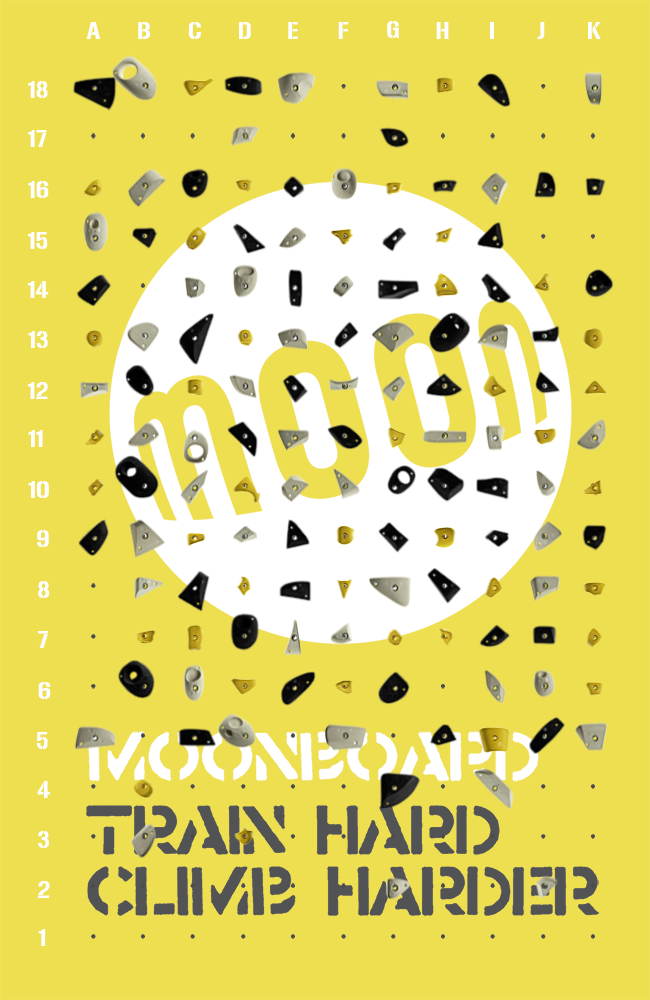
\includegraphics[width=.6\linewidth]{moonboard_stock}
  \caption{Stock Moonboard 2016 configuration}
  \label{fig: Stock Moonboard}
\end{subfigure}
\begin{subfigure}{.48\textwidth}
  \centering
  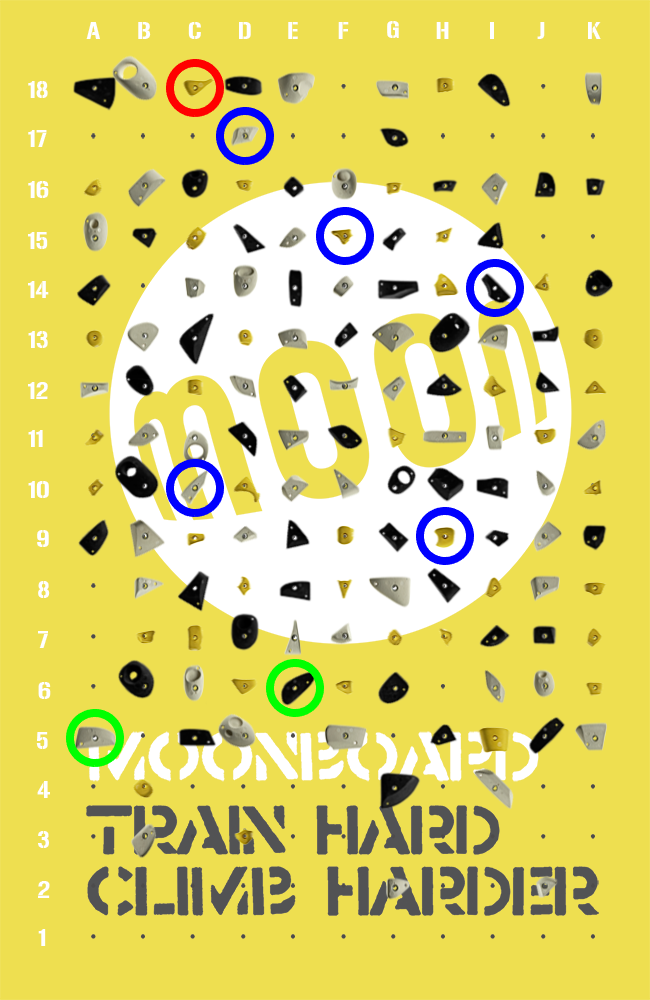
\includegraphics[width=.6\linewidth]{moonboard_1}
  \caption{A specific Moonboard problem}
  \label{fig: Moonboard Problem}
\end{subfigure}
\caption{Moonboard training apparatus showing a specific Moonboard problem}
\end{figure}

\begin{figure}
\centering
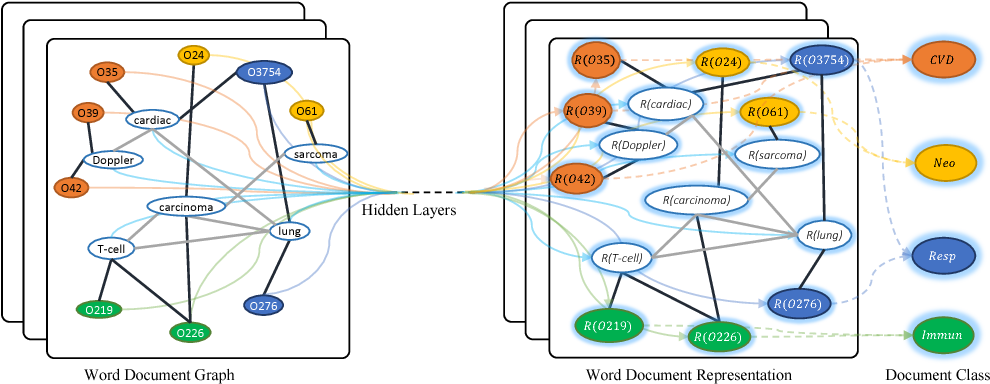
\includegraphics[width=.7\linewidth]{textGCN}
\caption{A heterogenous corpus graph for document classification using a Text Graph Convolutional Network [3]. Nodes come in 2 types: document entities and word entities. The different colors correspond to different node categories (notice only document nodes are colored). A direct analogy to Moonboard problems can be made by substituting documents for problems and holds for nodes.}
\label{fig: Corpus graph for Text Graph Convolutional Network}
\end{figure}

\section{Preprocessing and Modeling}
We successfully mined over 13,000 labeled problems from Moonboard's website. To transform our scraped data into a modeling-friendly format, we took two approaches: (1) representing both problems and holds as one-hot vectors and (2) encoding problems as multi-hot vectors and holds as one-hot vectors. Approach (1) was directly taken from the authors of [3] whose graph-creation strategy is summarized in Figure 2. Edges in that graph were represented using an adjacency matrix which we've adapted to the following form:

\[
    A_{ij}= 
\begin{cases}
    \text{PMI}(i, j), & \text{if } i, j \text{ holds} \\
    \text{IDF}(j), & \text{if } i \text{ problem } j \text{ hold} \\
    1, & \text{if } i=j \\
    0, & \text{otherwise}
\end{cases}
\]

In the above equation, \texttt{PMI} refers to \textit{Pointwise-Mutual Information} --- a metric that measures the degree of independence between two random variables and in our context can be interpreted as the log co-occurrence probability of holds. \texttt{IDF} refers to the \textit{Inverse Document Frequency} component of the famous \texttt{TFIDF} embedding strategy. While the authors of [3] used TFIDF in defining adjacency between words and documents, term frequency is redundant in our context since holds can never appear more than once in a single Moonboard route.

On the modeling side, we've implemented a baseline logistic regression classifier using feature set (2) along with a preliminary PyTorch implementation of the Text GCN [3] architecture using feature set (1) --- both models utilizing multi-class cross-entropy loss. Referencing Figure 1 which reports the baseline logistic regression model's performance metrics, we can see that this classification task is possible even for a simple LR model --- giving us confidence in continuing down the GCN route.

{\small\textbf{Code for logistic regression baseline model is \href{https://github.com/gestalt-howard/moonGen/tree/master/howard/models_baseline}{here}, preliminary GCN is \href{https://github.com/gestalt-howard/moonGen/tree/master/aaron/v0.0/scripts}{here}}}

\begin{figure}
\centering
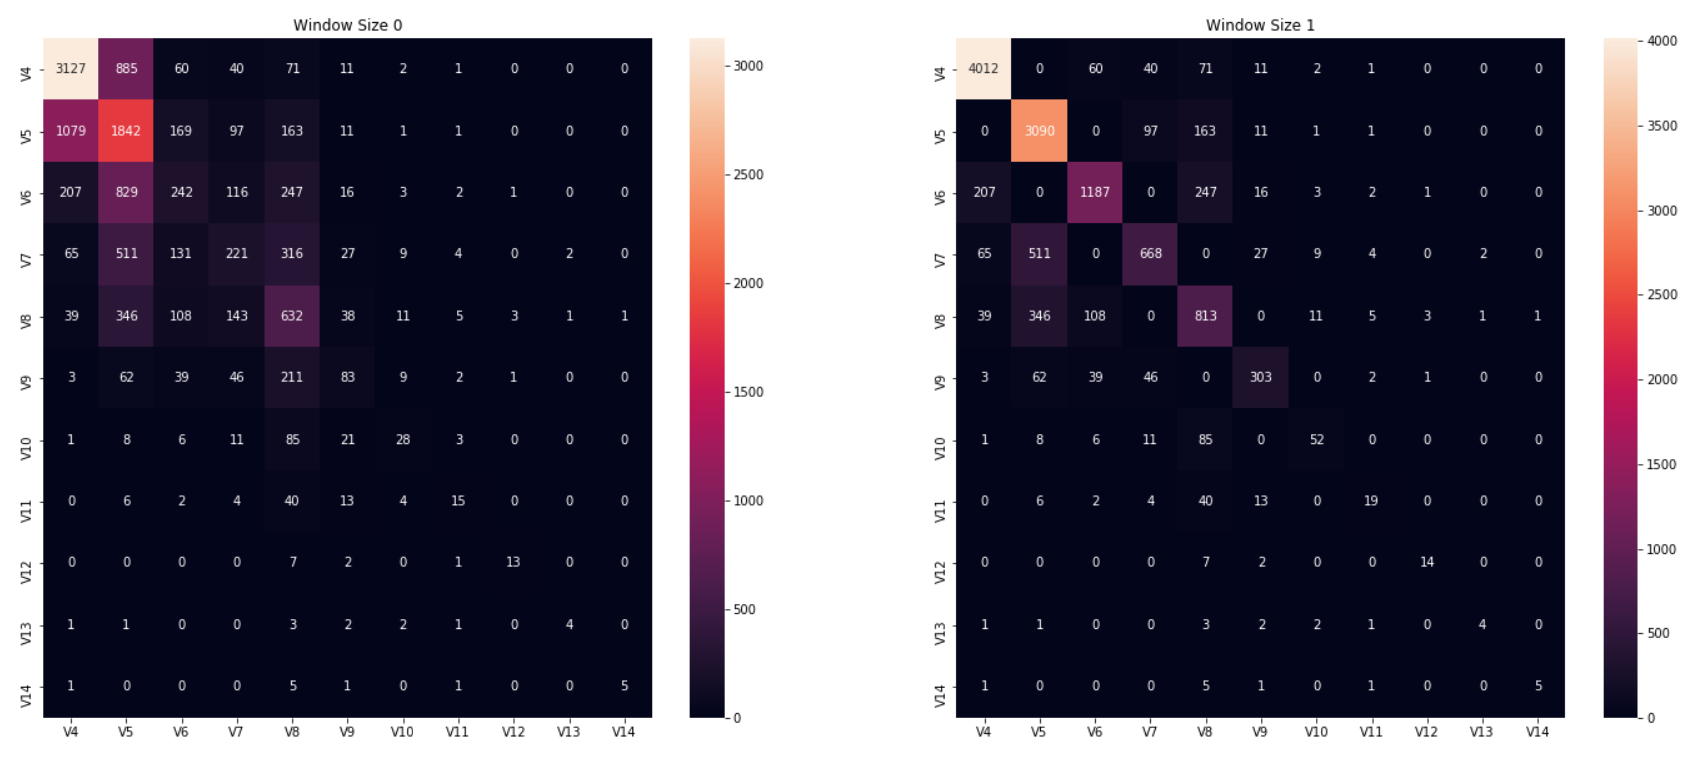
\includegraphics[width=.8\linewidth]{confusion_window}
\caption{Two confusion matrices that present a novel approach to model evaluation of a multi-category classifier. The left-hand plot shows a vanilla confusion matrix implementation (Window Size 0) while the right-hand matrix incorporates a sliding-window approach (Window Size 1) to determining false positive / true positive rates amongst the different difficulty classes.}
\end{figure}

\section{Evaluation Strategy}
To guide our decision-making throughout the remainder of this project, we invested significant effort in creating robust, custom evaluation metrics for monitoring model performance. Since our objective is multi-category classification, our evaluation strategy incorporates many proven classification-compatible metrics (i.e. F1-score, accuracy, recall, precision, AUC) along with confusion matrices and correlation plots. In addition, we extended each of these techniques to accomodate a sliding window over the difficulty classes. This custom addition encodes an intuition that we are willing to accept a \(+/- 1\) margin of error in our difficulty classification (i.e. a V4 problem can be mistaken for a V5 but not a V6, if using a sliding window size of 1). Altogether, these metrics are combined into three distinct visualizations (see Table 1) 

\begin{table}[h!]
	\begin{center}
		\begin{tabular}{c|c|c}
		\textbf{Plot Type} & \textbf{Description} & \textbf{Number of Plots}\\	
		\hline
		FARPA & F1, Accuracy, Precision, Recall, AUC for each class & 22\\
		Confusion & Confusion matrix with sliding windows & 2\\
		Correlation & Correlation plot with linear trend-fitting / p-value & 2\\
		\end{tabular}
	\vspace{0.01cm}
	\caption{Description of evaluation visualizations}
	\end{center}
\end{table}

{\small\textbf{Code for model evaluation can be found \href{https://github.com/gestalt-howard/moonGen/blob/master/howard/models_baseline/model_utils/evaluation_tools.py}{here}.}}

\section{Remaining Steps}
We plan on continuing to refine our GCN implementation by evaluating performance under different feature sets and adjacency definitions such that we are able to thoroughly characterize the behavior of our GCN model. Should we have additional time, we will explore a generative application [1] capable of producing a new Moonboard problem, given a user-specified difficulty.

\section*{References}
\medskip
\small

[1] Mirza, M. \& Osindero, S. \ Conditional Generative Adversarial Nets \ {\it arXiv:1411.1784} \ (2014)

[2] Wu, F., Zhang, T., de Souza Jr., A., Fifty, C., Yu, T., \& Weinberger, K. \ Simplifying Graph Convolutional Networks \ {\it Proceedings of the 36th International Conference on Machine Learning} \ (2019)

[3] Yao, L., Mao, C. \& Luo, Y. \ Graph Convolutional Networks for Text Classification \ {\it 33rd AAAI Conference on Artificial Intelligence (AAAI-19)}, 7370-7377 \ (2018)

\end{document}